\pdfoutput=1
\documentclass[11pt]{amsart}
\usepackage{amsmath,amssymb,amsthm,mathtools}
\usepackage[margin=1.2in]{geometry}
\usepackage{graphicx,booktabs,adjustbox,tikz}
\usetikzlibrary{arrows.meta,positioning,calc}
\usepackage{xcolor}
\usepackage[colorlinks=true,linkcolor=blue,citecolor=blue,urlcolor=blue]{hyperref}
\hypersetup{pdfauthor={Bernd Johannes Wuebben},pdftitle={Singular graded limits and metric growth under Hermitian--Yang--Mills flow}}
\setlength{\emergencystretch}{2em}
\newtheorem{theorem}{Theorem}[section]
\newtheorem{proposition}[theorem]{Proposition}
\newtheorem{lemma}[theorem]{Lemma}
\newtheorem{corollary}[theorem]{Corollary}
\theoremstyle{definition}
\newtheorem{definition}[theorem]{Definition}
\newtheorem{example}[theorem]{Example}
\newtheorem{question}[theorem]{Question}
\theoremstyle{remark}
\newtheorem{remark}[theorem]{Remark}
\newcommand{\CC}{\mathbb C}
\newcommand{\RR}{\mathbb R}
\newcommand{\ZZ}{\mathbb Z}
\newcommand{\PP}{\mathbb P}
\newcommand{\cO}{\mathcal O}
\newcommand{\cI}{\mathcal I}
\newcommand{\db}{\bar\partial}
\newcommand{\tr}{\operatorname{tr}}
\newcommand{\rk}{\operatorname{rk}}
\newcommand{\Hom}{\operatorname{Hom}}
\newcommand{\Coh}{\operatorname{Coh}}
\newcommand{\Vol}{\operatorname{Vol}}
\newcommand{\HYM}{\operatorname{HYM}}
\newcommand{\YM}{\operatorname{YM}}
\newcommand{\Gr}{\operatorname{Gr}}
\newcommand{\id}{\operatorname{id}}
\title[Singular graded limits and metric growth]{Singular graded limits and metric growth\\under Hermitian--Yang--Mills flow}
\author{Bernd Johannes Wuebben}
\subjclass[2020]{53C07 (primary); 32Q15, 14M25, 58E15 (secondary)}
\keywords{Hermitian--Yang--Mills flow, singular graded sheaf, weight filtration,
Hermitian--Einstein metric, curvature concentration, toric surface}
\date{October 31, 2026\\This version: October 31, 2026}

\begin{document}
\begin{abstract}
We construct a semistable toric tangent bundle for which the
weight-filtration description of Hermitian--Yang--Mills metric growth
cannot extend to singular graded sheaves with a uniformly bounded
remainder. The bundle lies on a smooth projective surface, and its
Jordan--H\"older graded sheaf is singular at one point. For every smooth
initial metric with fixed Hermitian--Einstein determinant, the induced
squared norm on its unique saturated equal-slope line subsheaf is
$o(T^{-1/2})$ as the flow time $T$ tends to infinity, uniformly on compact
subsets away from that point. The rank-polarized iterated weight
filtration of Haiden--Katzarkov--Kontsevich--Pandit instead assigns the
scale $T^{-1/2}$, with no further nonzero weights. A splitting-independent
local residue forces divergent normalized extension energy, which an
exact dissipation identity converts into the strict decay estimate.
Approaching the wall from the stable side, we also identify the
Hermitian--Einstein limit with the reflexive graded bundle and locate
its multiplicity-one curvature concentration at the same point.
\end{abstract}

\maketitle


% Source: sections/01_introduction.tex
\section{Introduction}\label{sec:introduction}

The Hermitian--Yang--Mills flow on a semistable holomorphic bundle
approaches its polystable graded object at the level of connections,
allowing curvature concentration where the graded sheaf is singular.
The behavior of the Hermitian metric contains further information.
Even when the limiting connection is understood, the metric can diverge
along the complex gauge orbit, and the rates of this divergence distinguish
extensions with the same graded factors.

Haiden--Katzarkov--Kontsevich--Pandit describe these rates for semistable
quiver representations and for bundles on compact Riemann surfaces by
an iterated weight filtration \cite{hkkp2023,hkkp2018}. Lam extends this
description to semistable bundles with locally free Jordan--H\"older
graded object \cite[Theorems~1.1, 8.2]{lam2026}. In that setting the
weights give an asymptotic model with bounded error. The extension to
singular graded sheaves is explicitly anticipated in
\cite[Introduction and Remark~8.3]{lam2026}, using the quotient category
by sheaves supported in complex codimension at least two. A description
away from a codimension-two set is also anticipated in
\cite[Introduction]{hkkp2018}.

We give a smooth rank-two bundle on a compact K\"ahler surface for which
two precise bounded-remainder versions of that singular extension fail,
even on compact subsets away from the singular point. The categorical
weight filtration has only two weights and no later iterated term.
Nevertheless the logarithm of the induced line metric has an additional
unbounded negative discrepancy from the prescribed model. A local residue
at the singular point forces this discrepancy through a global
holomorphic-section identity.

\subsection{The flow theorem}
Let $X$ be the toric blowup of $\mathbb F_1$ with cyclic rays
\[
 (1,0),\ (1,1),\ (0,1),\ (-1,0),\ (1,-1).
\]
Write $S,f$ for the pullback section and fibre classes and $E$ for the
exceptional divisor. Its tangent bundle $V=T_X$ admits the saturated
sequence
\begin{equation}\label{eq:intro-extension}
 0\longrightarrow L\xrightarrow{\iota}V
 \longrightarrow\cI_pM\longrightarrow0,
 \qquad
 L=\cO_X(2S+f-E),\quad M=\cO_X(2f),
\end{equation}
where $p$ is the fixed point of the cone $((1,1),(0,1))$.
The ample class $\alpha_0=4S+7f-2E$ gives both factors degree $8$.
The bundle is strictly semistable, and its graded sheaf is
$L\oplus\cI_pM$. Its geometry is recalled in full in
Section~\ref{sec:geometry}.

Fix any K\"ahler form $\omega\in\alpha_0$, and Hermitian--Einstein
metrics $h_L,h_M$ on the two line bundles. Put
$h_{\det}=h_Lh_M$, $v_0=\int_X\omega^2/2=18$ and
$\kappa=8\pi/9$. For a smooth Hermitian initial metric $H_{\mathrm{in}}$
with determinant $h_{\det}$, consider the actual metric flow
\[
 H^{-1}\partial_T H=-2(i\Lambda_\omega F_H-\kappa I),
 \qquad H(0)=H_{\mathrm{in}}.
\]
The ratio $u(T)=\iota^*H(T)/h_L$ is a globally smooth nonnegative
function, positive on $U=X\setminus\{p\}$ and zero at $p$. Set
$Z(T)=\int_Xu(T)\,\omega^2/2$.

\begin{theorem}\label{thm:flow}
For every initial metric just specified and every compact $K\subset U$,
\begin{equation}\label{eq:intro-normalized}
 \frac{u(T)}{Z(T)}\longrightarrow\frac1{18}
       \quad\text{in }C^\infty(K),
\end{equation}
and
\begin{equation}\label{eq:intro-decay}
 \frac{-Z'(T)}{Z(T)^3}\longrightarrow+\infty,
 \qquad\sqrt T\,Z(T)\longrightarrow0.
\end{equation}
In particular $u(T)=o(T^{-1/2})$ uniformly on $K$. If $K$ is nonempty,
\begin{equation}\label{eq:intro-log}
 \sup_K\left(\log u(T)+\frac12\log T\right)\longrightarrow-\infty.
\end{equation}
The constants and convergence times may depend on the initial metric.
\end{theorem}

In the slope-$8$ part of $\Coh(X)/\Coh_0(X)$, the full subobject
lattice of $V$ is $0<L<V$. Its rank-polarized iterated weights are
$-1/2$ on $L$ and $+1/2$ on $M$, with all further weights zero
(Section~\ref{sec:weights}). These are squared-metric weights.
Thus Theorem~\ref{thm:flow} detects a discrepancy on exactly the line
to which the categorical model assigns the scale $T^{-1/2}$.

To state the bounded-remainder consequence precisely, choose a fixed
smooth splitting $\Psi:L\oplus M\to V|_U$ restricting to $\iota$ on
$L$, and let
\[
 G_T=\Psi_*(T^{-1/2}h_L\oplus T^{1/2}h_M),\qquad
 G_0=\Psi_*(h_L\oplus h_M).
\]
Let $A_T$ be the positive $G_0$-self-adjoint endomorphism representing
$H(T)$, and $P$ the $G_0$-orthogonal projection onto $\iota(L)$.

\begin{corollary}\label{cor:intro}
On no nonempty compact subset $K\subset U$ can either of the following
hold with a constant independent of $T$:
\begin{align}
 C_K^{-1}G_T&\le H(T)\le C_KG_T,\label{eq:intro-order}\\
 \left\|\log A_T-\tfrac12\log T\,(I-2P)\right\|_{G_0}
       &\le C_K.\label{eq:intro-matrix-log}
\end{align}
\end{corollary}

The first assertion follows by restricting the metric order to $L$.
For the second, spectral Jensen gives
$\langle e,A_Te\rangle\ge\exp\langle e,\log A_Te\rangle$ for a
$G_0$-unit vector in $L$; both proposed bounds would force a positive
multiple of $T^{-1/2}$ as a lower bound for $u$.
The full argument is in Section~\ref{sec:obstruction}.
The two matrix formulations are distinguished because ordinary matrix
logarithms and relative metric order need not agree in a noncommuting
problem.

The anticipated extension to singular graded sheaves does not specify a
topology for the bounded remainder.
Corollary~\ref{cor:intro} tests the two formulations displayed here;
it does not attribute either to a numbered singular-case conjecture.
The locally free graded theorem is unaffected. Nor does
\eqref{eq:intro-log} determine the limit of $\log u/\log T$: a leading
coefficient $-1/2$ with an additional unbounded, slower term remains
possible.

\subsection{Why a point singularity affects the metric away from it}
Locally at $p$, the inclusion and quotient are $(z_1,-z_2)^{\mathsf t}$
and $(z_2,z_1)$. On a punctured ball a smooth splitting has a Dolbeault
extension form $\beta$. Its residue is independent of the splitting and
nonzero. It follows that, in fixed smooth graded metrics,
\begin{equation}\label{eq:intro-residue}
 \int_{\rho<r<R}|\beta|_0^2\,dV
       \ge c(\rho^{-2}-R^{-2}).
\end{equation}
The same lower bound holds for the orthogonal splitting selected by
$H(T)$, despite its time dependence.

The global norm of the inclusion satisfies the exact identity
\[
 -Z'(T)=2\int_X|D'_{H(T)\otimes h_L^{-1}}\iota|^2\,dV.
\]
Fixing the determinant gives a cubic metric factor in the normal
component of this derivative. On every annulus,
\[
 \frac{-Z'(T)}{Z(T)^3}
 \ge2\int_{\rho<r<R}(u/Z)^3|\beta_T|_0^2\,dV.
\]
The normalized section has a uniform scalar bound. The known connection
limit of Sibley--Wentworth \cite{sibleywentworth2015}, together with
Hartogs extension, then gives $u/Z\to1/v_0$ off $p$.
First let $T\to\infty$ with $\rho$ fixed, and then let $\rho\to0$.
The residue makes $-Z'/Z^3$ tend to infinity, from which the strict
little-oh decay follows by integration. The proof requires no estimate
for the shrinking size of a region of curvature concentration.

\subsection{A complementary stationary limit}
The same example has a stable side. Set
$\alpha_t=4S+(7+t)f-2E$ for $-1<t<0$ and choose a smooth K\"ahler
family $\omega_t\in\alpha_t$ through $\omega_0=\omega$. Let $D_t$
be the actual Hermitian--Einstein connections on $V$, presented on one
fixed Hermitian bundle with smoothly varying determinant, and let
$F_t^0$ denote their trace-free curvature. At the wall put
$D_*=D_L\oplus D_M$.

\begin{theorem}\label{thm:stationary}
As $t\uparrow0$, the ideal unitary limit of $D_t$
is $(L\oplus M,D_*)$ together with the point $p$ of multiplicity one.
Every sequence has a subsequence converging smoothly modulo unitary gauge
on compact subsets of $X\setminus\{p\}$. The full curvature measures,
and likewise the trace-free curvature measures, converge with the atom
$8\pi^2\delta_p$. In particular,
\begin{equation}\label{eq:intro-energy}
 |F_t^0|_t^2dV_t\rightharpoonup|F_*^0|_0^2dV+8\pi^2\delta_p,
 \qquad
 \int_X|F_t^0|_t^2dV_t=26\pi^2,
 \quad\int_X|F_*^0|_0^2dV=18\pi^2.
\end{equation}
If $\Pi_t$ is the orthogonal projection onto the image of $L$, then
\begin{equation}\label{eq:intro-projection}
 \|\db_{D_t}\Pi_t\|_{L^2(dV_t)}^2=-2\pi t,
 \qquad
 \|i\Lambda_0F_{D_t}-\kappa I\|_{L^2(dV)}=O(|t|).
\end{equation}
\end{theorem}

The sheaf $L\oplus\cI_pM$ also occurs as the special fibre of a flat
family whose nonzero fibres are isomorphic to $V$.

Projectively anti-self-dual compactness supplies a reflexive bundle and
an integral point cycle. To identify them, normalize the original
holomorphic inclusion to have integral squared norm one. A scalar bound
retains its mass, and the limiting map is nonzero and parallel. This
forces the limiting bundle to be $L\oplus M$. Its second Chern number
leaves one point of concentration; the fact that every original inclusion
vanishes at $p$ forces that point to be $p$ itself.

The stationary proof also verifies the strengthened hypotheses in the
Daskalopoulos--Wentworth correction \cite{daskalopouloswentworth2007}
and reconciles the corresponding gauges with the smooth compactness
limit. The point cycle is necessary: $c_2(V)=5$ whereas
$c_2(L\oplus M)=4$, so there is no global smooth bundle isomorphism
between them.

\subsection{Relation to existing results and organization}
The toric construction and its stability wall are taken from
\cite{wuebben2026}, and are recalled to make the local singularity explicit.
The convergence of the actual flow to the reflexive graded connection,
including its singular set, is the theorem of Sibley--Wentworth in its
corrected form. Our flow result adds a quantitative obstruction for the
metric: its restriction to the canonical line is strictly smaller than
the categorical two-weight scale. The new use of the residue is uniform
in the changing splitting, which is what allows the connection limit
to be combined with the global dissipation identity.

Related normalized induced-metric estimates in
\cite[Theorem~3.5]{lzz2016} assume the strict slope gap imposed in that
paper's Section~3. The present equal-slope extension has no such gap.
We use its standard flow normalization and mean-curvature estimate,
not that separate induced-metric theorem.

Sections~\ref{sec:geometry} and \ref{sec:weights} give the example and
its complete weight calculation. Section~\ref{sec:residue} proves the
local residue estimate and its metric weight.
Sections~\ref{sec:flow}--\ref{sec:obstruction} prove
Theorem~\ref{thm:flow} and Corollary~\ref{cor:intro}.
Section~\ref{sec:stationary} proves Theorem~\ref{thm:stationary},
including its exact projection identity and the curvature measure.
The final section identifies the remaining quantitative question.

% Source: sections/02_geometry.tex
\section{A toric surface with a singular graded quotient}\label{sec:geometry}

We first describe the bundle and its semistability wall. This construction
appeared in \cite[Example~4.3]{wuebben2026}; the details below fix the local
maps and normalizations used in both analytic arguments.

\subsection{The surface and the polarization}
Let $X$ be the smooth complete toric surface with rays
\begin{equation}\label{eq:rays}
 v=(1,0),\quad w=(1,1),\quad b=(0,1),\quad -v=(-1,0),\quad b'=(1,-1)
\end{equation}
in cyclic order. Consecutive pairs span its maximal cones. Their determinants
are one, so $X$ is smooth. Removing the ray $w$ gives the fan of the first
Hirzebruch surface $\mathbb F_1$; thus $X$ is its blowup at the fixed point
of the cone $(v,b)$. We use $S$ and $f$ for the pullbacks of the negative
section and fibre classes, and $E$ for the exceptional divisor. The
intersection pairing is
\begin{equation}\label{eq:intersection}
 S^2=-1,\qquad S f=1,\qquad f^2=0,\qquad E^2=-1,\qquad SE=fE=0.
\end{equation}
The class of the polarization will be denoted by $\alpha_t$, leaving $H$
for a Hermitian metric:
\begin{equation}\label{eq:polarization}
 \alpha_t=4S+(7+t)f-2E.
\end{equation}
Here $t$ is a real parameter. Flow time will always be denoted by $T$.

In the ray order $(v,-v,b,b',w)$ a divisor representing $\alpha_t$ has
coefficients $(4,0,0,7+t,2)$. Its polygon is
\[
 -4\le x\le0,\qquad 0\le y\le x+7+t,\qquad x+y\ge-2.
\]
For $t>-1$ the vertices are
\[
 (-4,2),\quad(-2,0),\quad(0,0),\quad(0,7+t),\quad(-4,3+t).
\]
Every edge has positive lattice length, and the normal fan is the fan
of $X$. Thus $\alpha_t$ is ample. The degrees of the invariant divisors
are respectively
\begin{equation}\label{eq:divisor-degrees}
 (1+t,\,7+t,\,2,\,4,\,2).
\end{equation}
The same calculation shows that this path leaves the ample cone at
$t=-1$.

\begin{figure}[htbp]
\centering
\begin{adjustbox}{max width=\textwidth,center}
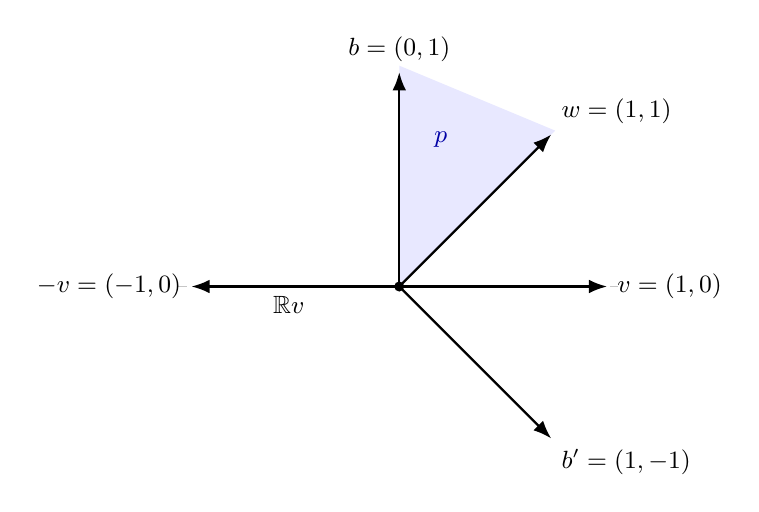
\begin{tikzpicture}[scale=1.65,>=Latex,font=\small]
\fill[blue!9] (0,0)--(1.2,1.2)--(0,1.7)--cycle;
\draw[gray!45,dashed] (-1.7,0)--(1.7,0);
\draw[->,thick] (0,0)--(1.6,0) node[right] {$v=(1,0)$};
\draw[->,thick] (0,0)--(1.17,1.17) node[above right] {$w=(1,1)$};
\draw[->,thick] (0,0)--(0,1.65) node[above] {$b=(0,1)$};
\draw[->,thick] (0,0)--(-1.6,0) node[left] {$-v=(-1,0)$};
\draw[->,thick] (0,0)--(1.17,-1.17) node[below right] {$b'=(1,-1)$};
\fill (0,0) circle (1.1pt);
\node[blue!65!black] at (.32,1.13) {$p$};
\node[below] at (-.85,0) {$\RR v$};
\end{tikzpicture}
\end{adjustbox}

\caption{The fan of $X$. The added ray $w$ subdivides the cone $(v,b)$
to give the blowup. The shaded cone $(w,b)$ corresponds to the point $p$
where the graded quotient is singular. The line $\RR v$ determines the
saturated tangent subsheaf.}
\label{fig:fan}
\end{figure}

\subsection{The saturated tangent line}
For a toric tangent bundle, a vector subspace $W$ of the torus Lie algebra
defines an equivariant saturated subsheaf whose first Chern class is the
sum of the invariant divisors with ray in $W$. The toric stability
criterion tests these subsheaves; see \cite{klyachko1990,hering2022}.
In dimension two it suffices to consider lines. Lines containing no ray
have degree zero. Among the ray lines, $\CC v$ contains both $v$ and
$-v$, whereas each of the other three contains only one ray.

Consequently their degrees are $8+2t$, $2$, $4$ and $2$. The tangent
bundle $V=T_X$ has slope
\begin{equation}\label{eq:slopes}
 \mu_t(V)=8+t.
\end{equation}
It is slope stable for $-1<t<0$, strictly semistable at $t=0$, and
unstable for $t>0$. At $t=0$ the unique equality among these tests is
$\CC v$.

The saturated rank-one subsheaf for this line is
\begin{equation}\label{eq:line-bundles}
 L=\cO_X(2S+f-E),\qquad M=\cO_X(2f).
\end{equation}
To see its class directly, the divisors of $v$ and $-v$ have classes
$S-E$ and $S+f$. Their sum is $c_1(L)$. A saturated rank-one subsheaf
of a locally free sheaf on a smooth surface is reflexive and hence a
line bundle. The determinant of $V$ is $\cO_X(2S+3f-E)=L\otimes M$.

Write $p$ for the fixed point of $(w,b)$. In the corresponding affine
chart, $v=w-b$, so the invariant vector field has expression
$z_1\partial_{z_1}-z_2\partial_{z_2}$. The saturated inclusion and
quotient are therefore
\begin{equation}\label{eq:local-resolution}
 0\longrightarrow\cO\xrightarrow{\;\iota=(z_1,-z_2)^{\mathsf t}\;}
 \cO^2\xrightarrow{\;q=(z_2,z_1)\;}(z_1,z_2)\longrightarrow0.
\end{equation}
The kernel assertion follows, for example, by comparing coefficients
in $z_2 a+z_1 b=0$: the regular sequence $z_1,z_2$ implies
$(a,b)=c(z_1,-z_2)$. The quotient is the maximal ideal of the origin.
Every other maximal cone contains a ray in $\RR v$. Saturation there
removes the divisorial zero of the invariant vector field, leaving a
nowhere-vanishing local generator. Thus $p$ is the sole zero of $\iota$.
Globally we obtain
\begin{equation}\label{eq:extension}
 0\longrightarrow L\xrightarrow{\iota}V
 \longrightarrow\cI_p M\longrightarrow0.
\end{equation}
We also use $q$ for the composite map $V\to\cI_pM\hookrightarrow M$.
In particular, $q_p$ is the zero map on fibres.

Both factors in \eqref{eq:extension} have slope $8$ at the wall and
are stable, being torsion-free of rank one. Hence the Jordan--H\"older
graded sheaf and its reflexive hull are
\begin{equation}\label{eq:graded}
 G=L\oplus\cI_pM,\qquad G^{**}=L\oplus M,
 \qquad G^{**}/G\simeq\CC_p\otimes M_p.
\end{equation}
The distinction between a saturated subsheaf and a subbundle matters here:
$L$ is locally free, but its inclusion into $V$ is not a subbundle
inclusion at $p$.

\subsection{Degrees, volume and curvature conventions}
All intersections below follow from \eqref{eq:intersection}:
\begin{equation}\label{eq:chern-data}
\begin{gathered}
 L^2=-1,\quad M^2=0,\quad LM=4,\quad c_1(V)^2=7,\quad c_2(V)=5,\\
 \deg_t L=8+2t,\quad\deg_t M=8,\quad
 \alpha_t^2=36+8t.
\end{gathered}
\end{equation}
Here $c_2(T_X)=5$ is also the number of two-dimensional cones in the fan.
In particular $c_2(L\oplus M)=4$: passing to the reflexive graded bundle
loses one unit of second Chern class.

Fix a K\"ahler form $\omega=\omega_0$ representing $\alpha_0$. The
volume form is $dV=\omega^2/2$ and
\begin{equation}\label{eq:volume}
 v_0=\Vol(X,\omega)=18,\qquad
 \kappa=\frac{2\pi\deg_0L}{v_0}=\frac{8\pi}{9}.
\end{equation}
Degrees mean $\int_X c_1(\,\cdot\,)\wedge\omega$, without division by volume.
Choose Hermitian--Einstein line metrics $h_L,h_M$ and put
$h_{\det}=h_Lh_M$. Their mean curvatures are both $\kappa$.
Constant rescaling of either line metric changes neither line connection.

On skew-Hermitian endomorphisms we use the inner product
$-\tr(AB)$, and on Hermitian endomorphisms we use $\tr(AB)$.
Form norms are the ordinary norms of the K\"ahler metric, and all integral
norms use the unnormalized volume. These conventions fix both the factor
$2$ in the metric flow and the energy $8\pi^2$ of an integral point defect.
The explicitly Euclidean coefficient norm used in the local residue
calculation will be specified separately.

% Source: sections/03_weights.tex
\section{The categorical weights at the wall}\label{sec:weights}

The singularity disappears from the graded factors when sheaves supported
at finitely many points are set equal to zero. The extension itself does
not split in that category. We determine its full subobject lattice,
including nonequivariant subobjects, before calculating its weights.

Let $\Coh_0(X)$ be the Serre subcategory of zero-dimensional coherent
sheaves. We work in the abelian category $\mathcal C$ of slope-semistable
objects of slope $8$ in $\Coh(X)/\Coh_0(X)$. Equivalently, one considers
semistable torsion-free sheaves of that slope, identifying modifications
at finitely many points and taking kernels and cokernels in the quotient
category. Divisorial torsion is not set equal to zero. The finite-slope
condition excludes it from $\mathcal C$. Rank is a positive additive
function on nonzero objects of $\mathcal C$.

This is the category appropriate to the rank-polarized weight filtration
in the singular surface case; compare \cite[Remark~8.3]{lam2026} and
\cite[\S4.1, equation~(4.3)]{hkkp2018}. Formula \eqref{eq:extension} becomes an extension
of $M$ by $L$ in $\mathcal C$.

\begin{lemma}\label{lem:lattice}
The subobject lattice of $V$ in $\mathcal C$ is the three-element chain
$0<L<V$. Its simple constituents are the distinct rank-one objects $L$
and $M$, and the extension does not split in $\mathcal C$.
\end{lemma}

\begin{proof}
A rank-one torsion-free sheaf on a smooth surface has a line bundle as its
double dual. It differs from that line bundle only at finitely many points,
so they define the same object in $\mathcal C$. A same-rank subobject of
the same degree can differ from it only by a zero-dimensional quotient:
a nonempty effective divisor has positive degree against an ample class.
It follows that a rank-one object of $\mathcal C$ is simple.

We shall also need the fact that a morphism between vector bundles in
$\Coh(X)/\Coh_0(X)$ is represented by an ordinary global bundle map.
Indeed, after modifying its source at finitely many points, such a morphism
is an ordinary map off that finite set; a vector-bundle target has no
zero-dimensional subsheaf. In local frames its coefficients extend across
the missing points by Hartogs' theorem, and the extensions agree by
uniqueness. This proves the assertion, including uniqueness of the
representative.

A nonzero map between distinct line bundles of equal degree cannot exist.
Its zero divisor would be effective of degree zero and hence empty,
which would make the map an isomorphism. Thus
$\Hom(L,M)=\Hom(M,L)=0$.

If the extension split in $\mathcal C$, its right inverse would be a map
$s:M\to V$. By the preceding Hartogs argument it would extend to a
holomorphic bundle map on $X$. The identity $qs=\id_M$, valid away from
finitely many points, would then hold everywhere. At $p$ this contradicts
$q_p=0$.

Finally, any proper nonzero subobject $A$ of $V$ has rank one. If
$A\ne L$, simplicity gives $A\cap L=0$, and the composite $A\to V\to M$
is a nonzero map between simple objects. It is an isomorphism and would
split the extension. This is impossible, so $L$ is the only such subobject.
\end{proof}

\begin{proposition}\label{prop:weights}
The rank-polarized iterated weight filtration of $V$ assigns weight
$-\tfrac12$ to $L$ and $+\tfrac12$ to $M$. All subsequent iterated
weights vanish.
\end{proposition}

\begin{proof}
The polarized chain in Lemma~\ref{lem:lattice} is the subobject lattice
of the two-vertex representation with one nonzero arrow $M\to L$ and
unit masses at the vertices. In the construction of
Haiden--Katzarkov--Kontsevich--Pandit, the weight filtration depends only
on this polarized lattice \cite[\S\S3.1,3.3,4.3]{hkkp2023}.
Here it minimizes
\[
 w_L^2+w_M^2\quad\text{subject to}\quad w_M-w_L\ge1.
\]
The minimum occurs at $w_L=-1/2$, $w_M=1/2$.

To check that there is no further iterated contribution, one must also
perform the next lattice construction. Its elements are pairs $(A,B)$
with $A\in[0,L]$ and $B\in[L,V]$ such that the interval $[A,B]$ is
complemented. Here an interval is complemented if each of its elements
has a lattice complement; for subobjects this is the condition of
semisimplicity. The two entries record the choices in the two successive
weight intervals. The derived lattice therefore has three elements,
\[
 (0,L),\qquad (L,L),\qquad (L,V).
\]
The pair $(0,V)$ is excluded because the interval $[0,V]$ is not
complemented: the middle element $L$ has no complement. With the charges
measured from the least element, the charge of $(A,B)$ is
\[
 (1-i/2)\rk A+(1+i/2)(\rk B-\rk L).
\]
Thus its real part records rank, and its imaginary part records rank
weighted by the first filtration weights. The three charges are
\[
 0,\qquad 1-\frac{i}{2},\qquad 2.
\]
Phase is the argument of a nonzero charge. Among nonzero elements,
only the greatest element has phase zero. Retaining the least element
by convention therefore leaves a two-element complemented lattice. Its weight filtration is
trivial, and so are all subsequent iterations. This is the iteration
specified in \cite[\S\S4.4--4.5]{hkkp2023}.
\end{proof}

The normalization in Proposition~\ref{prop:weights} is the normalization
for squared metric norms. In the two-vertex solution of
\cite[Example~5.12, equations~(5.104)--(5.106)]{hkkp2023}, the source
metric grows as $T^{1/2}$ and the target metric decays as $T^{-1/2}$.
Taking a square root would instead describe the norm of a frame, and
would change these exponents by a factor of two.

There is a useful analytic interpretation of the same calculation.
Suppose the orthogonal line metric were $a(T)h_L$, with determinant fixed.
The quotient metric would be $a(T)^{-1}h_M$, and the squared norm of an
extension form, measured in these metrics, would acquire a factor $a(T)^2$.
If its energy relative to the fixed line metrics were a positive finite
constant $c$, the line-norm dissipation would have cubic size $ca(T)^3$.
The scalar equation $-a'=ca^3$ gives $a(T)\asymp T^{-1/2}$.
This explains the scale appearing in the weight calculation. In our
example every fixed-metric extension form has infinite energy near $p$.
The next section proves that assertion in a form uniform over all
splittings, which will allow its use for the moving orthogonal splitting
of the actual flow.

% Source: sections/04_residue.tex
\section{The local extension form and its residue}\label{sec:residue}

The local sequence \eqref{eq:local-resolution} splits smoothly on a punctured
ball. Its Dolbeault extension form depends on that splitting, but one of
its integrals does not. This invariant integral is the analytic obstruction
we shall use.

\subsection{An explicit splitting}
Work on $B_R\subset\CC^2$ in the coordinates of
\eqref{eq:local-resolution}, and put $r^2=|z_1|^2+|z_2|^2$.
A smooth right inverse of $q$ on $B_R\setminus\{0\}$ is
\begin{equation}\label{eq:lift}
 \tau_0=\frac1{r^2}\begin{pmatrix}\overline z_2\\\overline z_1\end{pmatrix}.
\end{equation}
The two-column frame $(\iota,\tau_0)$ has determinant one. Since
$q\tau_0=1$ and $q$ is holomorphic, $\db\tau_0$ lies in the line
spanned by $\iota$. Direct differentiation gives
\begin{equation}\label{eq:beta}
 \db\tau_0=\iota\beta_0,
 \qquad \beta_0=\frac{\overline z_1\,d\overline z_2-
                      \overline z_2\,d\overline z_1}{r^4},
 \qquad \db\beta_0=0.
\end{equation}
For instance the $d\overline z_1$ coefficient of $\db\tau_0$ is
$(-z_1\overline z_2,|z_2|^2)^{\mathsf t}/r^4$, which is
$\iota(-\overline z_2/r^4)$. The other coefficient is obtained in the
same way.

For this calculation only, give $d\overline z_1,d\overline z_2$ unit
coefficient norm, and use Lebesgue volume on $\RR^4$. Then
\begin{equation}\label{eq:beta-energy}
 |\beta_0|^2=r^{-6},\qquad
 \int_{\rho<r<R}|\beta_0|^2\,dV_{\mathrm{Euc}}
 =\pi^2(\rho^{-2}-R^{-2}).
\end{equation}
The divergence is therefore stronger than logarithmic. Merely choosing a
different splitting might conceivably change this conclusion. The residue
rules out that possibility.

\begin{lemma}\label{lem:residue}
For every smooth right inverse $\tau$ of $q$ on $B_R\setminus\{0\}$,
write $\db\tau=\iota\beta_\tau$. There is $c>0$, independent of $\tau$
and of $0<\rho<R$, such that
\begin{equation}\label{eq:residue-energy}
 \int_{\rho<r<R}|\beta_\tau|^2\,dV_{\mathrm{Euc}}
 \ge c(\rho^{-2}-R^{-2}).
\end{equation}
The conclusion also holds with fixed smooth base and line metrics that
extend positively to a neighborhood of the closed ball, with a different
constant $c$.
\end{lemma}

\begin{proof}
On the punctured ball any two right inverses differ by a multiple of
$\iota$. Thus $\tau=\tau_0+\iota f$ for a smooth function $f$, and
\begin{equation}\label{eq:change-splitting}
 \beta_\tau=\beta_0+\db f.
\end{equation}
Let $S_r$ have the outward boundary orientation. The form
$dz_1\wedge dz_2\wedge\beta_0$ restricts to twice $r^{-3}$ times the
oriented Euclidean area form. One can check this at $(r,0)$ and use
$U(2)$ invariance; the determinant factor of $dz_1\wedge dz_2$ is
cancelled by the conjugate determinant factor in $\beta_0$. Since
$\operatorname{area}(S_r)=2\pi^2 r^3$, we obtain
\begin{equation}\label{eq:residue}
 \int_{S_r}dz_1\wedge dz_2\wedge\beta_0=4\pi^2.
\end{equation}
For completeness, at $(r,0)$ the form is
$r^{-3}dz_1\wedge dz_2\wedge d\overline z_2$; on the positively
oriented tangent frame in the $y_1,x_2,y_2$ directions it equals
$2r^{-3}$.

The change in the integrand under \eqref{eq:change-splitting} is
$d(f\,dz_1\wedge dz_2)$. Its integral over the sphere is zero.
Hence \eqref{eq:residue} holds with $\beta_\tau$ in place of $\beta_0$.
Restriction to $S_r$ and Cauchy--Schwarz now give
\[
 4\pi^2
 \le C\int_{S_r}|\beta_\tau|\,dA
 \le C(2\pi^2r^3)^{1/2}
          \left(\int_{S_r}|\beta_\tau|^2\,dA\right)^{1/2}.
\]
Thus the spherical integral is bounded below by $c_1r^{-3}$.
Integration in $r$ proves \eqref{eq:residue-energy}. Fixed smooth positive
metrics on the closed ball are uniformly equivalent to these Euclidean
norms and volume, proving the final assertion.
\end{proof}

In particular there is no smooth splitting whose extension form is
square-integrable near the origin in fixed smooth graded metrics.
The uniformity over splittings is essential: the orthogonal splitting
selected by the evolving metric will vary with time, and we have no
uniform bound on its derivatives near the singular point.

\subsection{The metric factor in the extension energy}
Fix the metrics $h_L,h_M$ from Section~\ref{sec:geometry}. For a smooth
Hermitian metric $H$ on $V$ with determinant $h_{\det}$, define
\begin{equation}\label{eq:u-metric}
 u_H=\frac{\iota^*H}{h_L}.
\end{equation}
This is a smooth nonnegative function on $X$, vanishing precisely at $p$.
On $U=X\setminus\{p\}$ use the $H$-orthogonal right inverse $\tau_H$
of $q$. The induced line and quotient metrics in this splitting are
\begin{equation}\label{eq:orthogonal-metrics}
 u_H h_L,\qquad u_H^{-1}h_M.
\end{equation}
Indeed their product is the fixed determinant metric, and the frame
$(\iota,\tau_H)$ is compatible with the determinant identification.

Write $|\beta_H|_0$ for the norm using the fixed line metric
$h_Lh_M^{-1}$ and the fixed base form $\omega$. From
\eqref{eq:orthogonal-metrics} the norm using the actual induced metrics
satisfies
\begin{equation}\label{eq:weighted-beta}
 |\beta_H|_H^2=u_H^2|\beta_H|_0^2.
\end{equation}
Let $\Pi_H$ be the orthogonal projection onto $\iota(L)$ on $U$.
In the orthogonal splitting, $\db\Pi_H$ has the off-diagonal block
$\beta_H$ up to sign, so
$|\db\Pi_H|^2=|\beta_H|_H^2$.

Regard $\iota$ as a holomorphic section of $V\otimes L^{-1}$. Its
normal covariant derivative is obtained by applying the adjoint
$(1,0)$ off-diagonal block to that section. The section itself has
squared norm $u_H$. The tangential and normal components of the derivative
are orthogonal. Consequently
\begin{equation}\label{eq:cubic}
 |D'_{H\otimes h_L^{-1}}\iota|^2
 \ge u_H|\beta_H|_H^2=u_H^3|\beta_H|_0^2.
\end{equation}
There are three factors of $u_H$: two from the Hom metric and one from
the norm of the section. This cubic weight is what connects the residue
to the scalar decay rate.

For each fixed smooth $H$, the local resolution implies $u_H\asymp r^2$
near $p$, with constants depending on $H$. Thus the fixed-metric
divergence of $\beta_H$ does not mean that the actual weighted quantities
in \eqref{eq:weighted-beta} or \eqref{eq:cubic} are infinite at a finite
time. The obstruction arises after normalization and passage to the
large-time limit.

% Source: sections/05_flow.tex
\section{The line inclusion along the metric flow}\label{sec:flow}

Let $H(T)$ solve
\begin{equation}\label{eq:flow}
 H^{-1}\partial_T H=-2\Phi_H,
 \qquad\Phi_H=i\Lambda_\omega F_H-\kappa I,
 \qquad H(0)=H_{\mathrm{in}},
\end{equation}
where $H_{\mathrm{in}}$ is any smooth positive Hermitian metric with
$\det H_{\mathrm{in}}=h_{\det}$. Long-time existence is the standard
Hermitian--Yang--Mills heat-flow theorem \cite{donaldson1985}.
The scalar determinant flow starts at its Hermitian--Einstein metric;
uniqueness for that scalar equation gives
$\det H(T)=h_{\det}$ for every $T\ge0$.

We use the intrinsic functions
\begin{equation}\label{eq:u-z}
 u(T,x)=\frac{\iota^*H(T)}{h_L}(x),
 \qquad Z(T)=\int_X u(T,x)\,dV.
\end{equation}
Although the orthogonal splitting is singular at $p$, the section
$\iota$ is globally smooth and holomorphic. In particular $Z(T)>0$
for every finite $T$, and its derivative can be computed on the entire
compact surface without introducing a puncture.

\subsection{Dissipation and a scalar bound}
\begin{lemma}\label{lem:dissipation}
For every $T\ge0$,
\begin{equation}\label{eq:dissipation}
 Z'(T)=-2\int_X|D'_{H(T)\otimes h_L^{-1}}\iota|^2\,dV\le0.
\end{equation}
There is a constant $C$, depending on $H_{\mathrm{in}}$ and the fixed
geometry but not on $T$, such that
\begin{equation}\label{eq:scalar-bound}
 \sup_X u(T,\cdot)\le C Z(T).
\end{equation}
\end{lemma}

\begin{proof}
The curvature contraction on $V\otimes L^{-1}$ is $\Phi_H$, because
$i\Lambda F_{h_L}=\kappa$. Differentiating the norm of the fixed section
along \eqref{eq:flow} gives
\[
 \partial_Tu=-2\langle\Phi_H\iota,\iota\rangle.
\]
For a holomorphic section the integrated K\"ahler Bochner identity is
\[
 \int_X\langle i\Lambda F_{V\otimes L^{-1}}\iota,\iota\rangle\,dV
 =\int_X|D'_{H\otimes h_L^{-1}}\iota|^2\,dV.
\]
The section and the bundle metric are smooth at $p$, so integration
introduces no singular boundary term. This proves
\eqref{eq:dissipation}.

With the real Laplacian $\Delta=2g^{j\bar k}\partial_j\partial_{\bar k}$,
the pointwise Bochner identity reads
\[
 \Delta u=2|D'_{H\otimes h_L^{-1}}\iota|^2
                -2\langle\Phi_H\iota,\iota\rangle.
\]
The mean-curvature maximum principle along \eqref{eq:flow} bounds
$\sup_X|\Phi_H(T)|_{H(T)}$ by its initial value. Its scalar heat
inequality follows by differentiating the contracted curvature along
the metric flow; in the present normalization
$(\partial_T-\Delta)|\Phi_H|^2\le0$.
The conventions and this inequality also appear in
\cite[equations~(1.5)--(1.6), (3.78)]{lzz2016}.
It follows that $\Delta u\ge-C_0u$, with $C_0$ independent of $T$.
The scalar mean-value estimate, or Moser iteration on the fixed compact
surface, now gives $\|u\|_{L^\infty}\le C\|u\|_{L^1}$.
This is \eqref{eq:scalar-bound}.
\end{proof}

Only the mean curvature is bounded in this argument. The full curvature
may concentrate at $p$, and the metric need not remain uniformly comparable
to a fixed smooth reference metric. The scalar estimate remains uniform
because its potential is measured in the current bundle metric and the
base geometry is fixed.

\subsection{The connection limit and normalized sections}
We use the corrected form of Sibley--Wentworth's convergence theorem
\cite[Theorem~1.1 and Remark~1.2]{sibleywentworth2015}. In the present
case it has the following content. After transporting the metric flow
to a fixed Hermitian bundle, the resulting Yang--Mills connections
converge modulo unitary gauge smoothly on compact subsets of
$U=X\setminus\{p\}$ to the Hermitian--Einstein connection on
$G^{**}=L\oplus M$. The algebraic singular set is $\{p\}$, with
multiplicity one. For the argument below, the subsequential formulation
along any sequence $T_j\to\infty$ suffices.

The hypotheses are satisfied: $X$ is compact K\"ahler, $V$ is a
holomorphic vector bundle, the initial metric is smooth, and
\eqref{eq:graded} is its graded sheaf at the fixed wall polarization.
Metric flow and connection flow are related by time-dependent complex
isometries and unitary gauge transformations. Those identifications
preserve the scalar norms of sections used here. In the chosen line
metrics the limiting connection is
\begin{equation}\label{eq:limit-connection}
 D_*=D_L\oplus D_M.
\end{equation}
We use normalized holomorphic inclusions to pass from this connection
convergence to information about the evolving metric.

\begin{proposition}\label{prop:normalized-flow}
For every compact $K\subset U$,
\begin{equation}\label{eq:normalized-flow}
 \frac{u(T,\cdot)}{Z(T)}\longrightarrow\frac1{v_0}
 \quad\text{in }C^\infty(K)\quad(T\to\infty).
\end{equation}
\end{proposition}

\begin{proof}
Transport $(V,H(T))$ isometrically to a fixed Hermitian bundle and
normalize the transported inclusion by $Z(T)^{-1/2}$. Denote the
resulting section of $V_T\otimes L^{-1}$ by $j_T$. It is holomorphic
for the transported Dolbeault operator and has global squared integral
norm one. Lemma~\ref{lem:dissipation} gives the pointwise bound
\begin{equation}\label{eq:normalized-bound}
 |j_T|^2=\frac{u(T)}{Z(T)}\le C.
\end{equation}

Choose any sequence $T_j\to\infty$. The preceding connection theorem
provides gauges in which the connections converge smoothly on compact
subsets of $U$. Interior elliptic estimates for the holomorphic section
equation, together with \eqref{eq:normalized-bound}, give bounds for all
derivatives of the sections on smaller compact sets. Passing to a diagonal
subsequence, we obtain a holomorphic limit
\[
 j_\infty\in H^0\bigl(U,(L\oplus M)\otimes L^{-1}\bigr).
\]
In holomorphic frames near $p$, its coefficients extend across the
puncture by Hartogs' theorem. It is therefore a global section of
$\cO_X\oplus(M\otimes L^{-1})$.

The second summand has no nonzero holomorphic section. Indeed it is a
nontrivial line bundle of degree zero; any nonzero section would define
an effective divisor of degree zero and hence trivialize it. It follows
that $j_\infty$ lies in the first summand and is constant there.
We still have to show that this constant is nonzero and determine its
norm. Smooth convergence off $p$ alone would not exclude concentration
of all the section's mass at $p$.

The pointwise bound does exclude that possibility. On any coordinate
ball $B_r(p)$,
\[
 \int_{B_r(p)}|j_{T_j}|^2\,dV\le C\Vol(B_r(p)),
\]
uniformly in $j$. Pass to the limit on $X\setminus B_r(p)$ and then
let $r\downarrow0$. Since the global integral is one, the limiting
section also has integral norm one. Its constant squared norm is
therefore $1/v_0$.

Finally, $|j_T|^2=u/Z$ is invariant under every isometry and unitary
gauge used above. Every sequence of times has a subsequence with the
same scalar $C^\infty$ limit on each compact subset. A subsequence
contradiction proves the full convergence \eqref{eq:normalized-flow}.
\end{proof}

The order of the preceding operations is useful to keep in mind.
Connection convergence gives a limiting holomorphic section away from
the singular set. The global scalar estimate retains its mass. Hartogs
extension and the equal-slope condition then identify it. No estimate
for the speed of connection convergence was needed.

% Source: sections/06_obstruction.tex
\section{Failure of the bounded metric asymptotics}\label{sec:obstruction}

We now combine the local residue with the global normalization. Their
combination forces an unbounded coefficient in the cubic dissipation
law, and this is stronger than a fixed multiple of the $T^{-1/2}$ decay predicted by the two-weight model.

\begin{proposition}\label{prop:faster-decay}
Along \eqref{eq:flow},
\begin{equation}\label{eq:divergent-dissipation}
 \frac{-Z'(T)}{Z(T)^3}\longrightarrow+\infty,
 \qquad \sqrt T\,Z(T)\longrightarrow0.
\end{equation}
Consequently, for every nonempty compact $K\subset U$,
\begin{equation}\label{eq:compact-decay}
 \sup_{x\in K}\sqrt T\,u(T,x)\longrightarrow0,
 \qquad
 \sup_{x\in K}\left(\log u(T,x)+\frac12\log T\right)
        \longrightarrow-\infty.
\end{equation}
\end{proposition}

\begin{proof}
Choose a coordinate ball whose closure lies in the chart of
\eqref{eq:local-resolution}. At each finite time, take the $H(T)$-orthogonal
right inverse of $q$ on the punctured ball, and denote its extension form
by $\beta_T$. In the fixed smooth line and base metrics,
Lemma~\ref{lem:residue} gives
\begin{equation}\label{eq:moving-residue}
 \int_{\rho<r<R}|\beta_T|_0^2\,dV
 \ge c(\rho^{-2}-R^{-2})
\end{equation}
for all $T$ and all $0<\rho<R$, with the same $c>0$.
Since the determinant is fixed, \eqref{eq:cubic} applies at every time.
Together with \eqref{eq:dissipation}, it gives
\begin{equation}\label{eq:normalized-dissipation}
 \frac{-Z'(T)}{Z(T)^3}
 \ge 2\int_{\rho<r<R}
       \left(\frac{u(T,x)}{Z(T)}\right)^3|\beta_T|_0^2\,dV.
\end{equation}

Fix $\rho>0$. Proposition~\ref{prop:normalized-flow} implies
$u(T)/Z(T)\ge1/(2v_0)$ on this closed annulus for all sufficiently
large $T$. Thus
\begin{equation}\label{eq:fixed-annulus-limit}
 \liminf_{T\to\infty}\frac{-Z'(T)}{Z(T)^3}
 \ge \frac{c}{4v_0^3}(\rho^{-2}-R^{-2}).
\end{equation}
The left-hand side is independent of $\rho$. Letting $\rho\downarrow0$
proves that it is $+\infty$.

It follows that
\[
 \frac{d}{dT}Z(T)^{-2}=-\frac{2Z'(T)}{Z(T)^3}\longrightarrow+\infty.
\]
For any $A>0$, this derivative is at least $A$ after some time $T_A$.
Integration yields
\[
 Z(T)^{-2}\ge Z(T_A)^{-2}+A(T-T_A)\qquad(T\ge T_A).
\]
After division by $T$ and passage to the limit, $\liminf Z(T)^{-2}/T\ge A$.
As $A$ is arbitrary, $\sqrt T\,Z(T)\to0$.
The uniform convergence of $u/Z$ on $K$ proves the first part of
\eqref{eq:compact-decay}. Its logarithm proves the second, since
$u(T,x)>0$ on $K$.
\end{proof}

The argument first lets time tend to infinity on a fixed annulus and
only then decreases its inner radius. It gives no uniform entry time
as that radius shrinks. In particular it neither selects a time-dependent
annulus nor estimates a bubble radius. This limit order is enough for
the strict little-oh conclusion.

\subsection{Two precise bounded-remainder assertions}
The weights in Proposition~\ref{prop:weights} lead to the following
candidate metric on the punctured surface. Choose any fixed smooth
filtration-compatible splitting
\[
 \Psi:L\oplus M\longrightarrow V|_U,
 \qquad \Psi|_L=\iota,
\]
and define, for $T\ge1$,
\begin{equation}\label{eq:model}
 G_T=\Psi_*(T^{-1/2}h_L\oplus T^{1/2}h_M).
\end{equation}
One possible bounded-remainder statement is bounded relative metric
order on compact subsets:
\begin{equation}\label{eq:order-claim}
 C_K^{-1}G_T\le H(T)\le C_KG_T\quad\text{on }K,
\end{equation}
with $C_K$ independent of $T$. The order is the order of positive
Hermitian forms on each fibre.

A second statement uses the ordinary logarithm of a positive matrix.
Let $G_0=\Psi_*(h_L\oplus h_M)$, write $A_T$ for the positive
$G_0$-self-adjoint endomorphism representing $H(T)$, and let $P$ be the
$G_0$-orthogonal projection onto $\iota(L)$. The proposed assertion is
\begin{equation}\label{eq:log-claim}
 \left\|\log A_T-\frac12\log T\,(I-2P)\right\|_{G_0}\le C_K
 \quad\text{on }K.
\end{equation}
Here the norm is the operator norm and the logarithm is defined by
spectral calculus. These two assertions should not be identified in a
noncommuting matrix problem.

\begin{corollary}\label{cor:two-obstructions}
Neither \eqref{eq:order-claim} nor \eqref{eq:log-claim} holds for any
nonempty compact $K\subset U$, for any fixed splitting $\Psi$ as above.
\end{corollary}

\begin{proof}
Restricting the lower inequality in \eqref{eq:order-claim} to $L$
would give $u(T,x)\ge C_K^{-1}T^{-1/2}$, contradicting
\eqref{eq:compact-decay}.

For \eqref{eq:log-claim}, fix a $G_0$-unit vector $e$ in $\iota(L)$.
The elementary spectral Jensen inequality gives
\begin{equation}\label{eq:jensen}
 u(T,x)=\langle e,A_Te\rangle_{G_0}
 \ge \exp\langle e,(\log A_T)e\rangle_{G_0}.
\end{equation}
Indeed, diagonalize $A_T$ and apply the scalar concavity of $\log$ to
the eigenvalues with weights given by the squared coefficients of $e$.
Since $Pe=e$, \eqref{eq:log-claim} implies that the last expression
is at least $e^{-C_K}T^{-1/2}$, again a contradiction.
\end{proof}

Thus the failure is detected by restriction to the canonical line. It
cannot be removed by altering the fixed smooth splitting or by passing
from metric order to the specified ordinary matrix-log formulation.
The argument does not infer either of those matrix assertions from the
other; it tests a necessary scalar inequality for each.

% Source: sections/07_stationary.tex
\section{Stationary degeneration and the curvature measure}\label{sec:stationary}

The same line inclusion identifies the limit of Hermitian--Einstein
connections as the polarization approaches the wall from the stable side.
Here the parameter is $t\uparrow0$, not flow time. We prove the compactness
and localization statement independently of the heat-flow convergence
used in Section~\ref{sec:flow}.

Retain the smooth K\"ahler family $\omega_t\in\alpha_t$ chosen in the
introduction, with $\omega_0=\omega$, and restrict to $-t_0\le t\le0$
for some $t_0\in(0,1)$. Such families exist: if $\eta$ is a smooth closed
real $(1,1)$-form representing $f$, then $\omega+t\eta$ is K\"ahler
for sufficiently small $|t|$. Linearity in $t$ is unnecessary below;
we use smooth dependence, the prescribed cohomology classes, and
$\Lambda_t-\Lambda_0=O(t)$ in smooth operator norms.
Write $dV_t=\omega_t^2/2$ and $\Lambda_t$ for contraction with
$\omega_t$. Then
\begin{equation}\label{eq:kappa-t}
 \Vol_t=18+4t,\qquad
 \kappa_t=\frac{2\pi(8+t)}{18+4t}.
\end{equation}
Let $h_{\det,t}$ be smoothly varying Hermitian--Einstein metrics on
$\det V$, chosen to agree with $h_{\det}$ at zero. Such a choice follows
from the scalar Poisson equation: normalize the logarithmic correction
to have zero $\omega$-mean, and use the smooth inverse of the Laplacian
on the complement of its constants. The mean-zero solvability condition
is precisely the degree identity.

For $t<0$ the bundle $V$ is stable. By the
Donaldson--Uhlenbeck--Yau theorem \cite{donaldson1985,uhlenbeckyau1986},
it has a Hermitian--Einstein metric $K_t$ with determinant $h_{\det,t}$.
Fix a smooth Hermitian metric $h$ on the underlying bundle with determinant
$h_{\det}$. Transport the Chern connection of $K_t$ through the positive
isometry $(V,K_t)\to(V,h)$ and denote the resulting unitary connection by
$D_t$. It satisfies
\begin{equation}\label{eq:he-t}
 F_{D_t}^{0,2}=0,
 \qquad i\Lambda_tF_{D_t}=\kappa_t I.
\end{equation}
Its Dolbeault operator lies in the complex gauge orbit of the fixed
holomorphic bundle $V$. Write $d_t$ for its determinant connection,
$f_t=\tr F_{D_t}$ for the determinant curvature, and
\begin{equation}\label{eq:trace-free}
 F_t^0=F_{D_t}-\tfrac12 f_t I
\end{equation}
for the trace-free curvature. The superscript $0$ in $F_t^0$ denotes the
trace-free part, not a form type. The connections $d_t$ and their curvatures
vary smoothly through $t=0$; no such assertion is made for $K_t$.

\subsection{The flat sheaf degeneration}
The algebraic degeneration is explicit. Write $s$ for the coordinate on
$\mathbb A^1$ and $\operatorname{pr}:X\times\mathbb A^1\to X$ for the
projection. Define
\begin{equation}\label{eq:flat-family}
 \mathcal V=\operatorname{coker}
 \left[\operatorname{pr}^*L\longrightarrow
       \operatorname{pr}^*V\oplus\operatorname{pr}^*L,
       \quad\ell\longmapsto(\iota\ell,-s\ell)\right].
\end{equation}
There is an exact sequence
\[
 0\longrightarrow\operatorname{pr}^*L\longrightarrow\mathcal V
 \longrightarrow\operatorname{pr}^*(\cI_pM)\longrightarrow0.
\]
For the injection, if $(0,\ell)$ lies in the image of the defining map,
injectivity of $\iota$ forces its preimage and $\ell$ to vanish. The
quotient assertion follows from \eqref{eq:extension}. Both end terms
are flat over $\mathbb A^1$, hence so is $\mathcal V$, and the sequence
remains exact on fibres. For $s\ne0$ the map
$[(e,\ell)]\mapsto e+s^{-1}\iota\ell$ identifies the fibre with $V$.
At $s=0$ the fibre is $L\oplus\cI_pM$.

Locally at $(p,0)$ the family has the presentation
\[
 \cO\xrightarrow{(z_1,-z_2,-s)^{\mathsf t}}\cO^3
       \longrightarrow\mathcal V\longrightarrow0.
\]
The loss of local freeness in the special fibre is visible in this
matrix. Its double dual has length-one quotient at $p$, as in
\eqref{eq:graded}. One may pair the real stable-side parameters by
$s=-t$, but flatness and the analytic limit below are distinct assertions.

\subsection{Quantitative curvature estimates}
\begin{proposition}\label{prop:stationary-energy}
The trace-free curvature has constant total energy
\begin{equation}\label{eq:energy26}
 \int_X|F_t^0|_t^2\,dV_t=26\pi^2.
\end{equation}
For a constant $C$ independent of $t\in[-t_0,0)$,
\begin{equation}\label{eq:wall-error}
 \|i\Lambda_0F_{D_t}-\kappa I\|_{L^2(dV)}\le C|t|.
\end{equation}
Moreover, with $\HYM_0(D)=\int_X|i\Lambda_0F_D|^2\,dV$,
\begin{equation}\label{eq:excess}
 \HYM_0(D_t)-2\kappa^2v_0
 =\|i\Lambda_0F_{D_t}-\kappa I\|_{L^2(dV)}^2\le C^2t^2.
\end{equation}
\end{proposition}

\begin{proof}
By \eqref{eq:he-t}, $F_t^0$ is a primitive $(1,1)$-form and is
therefore anti-self-dual on the K\"ahler surface. With the trace norm
fixed above, Chern--Weil gives
\[
 \int_X|F_t^0|_t^2\,dV_t
 =8\pi^2\left(c_2(V)-\frac14c_1(V)^2\right)
 =8\pi^2\left(5-\frac74\right)=26\pi^2.
\]
The determinant curvature is smooth, so the full curvature has uniformly
bounded integral squared norm as well. More explicitly, the surface
energy identity gives
\begin{equation}\label{eq:full-energy}
 \YM_t(D_t)
 =\HYM_t(D_t)+4\pi^2(2c_2(V)-c_1(V)^2)
 =\frac{8\pi^2(8+t)^2}{18+4t}+12\pi^2.
\end{equation}

The contraction operators satisfy $\|\Lambda_0-\Lambda_t\|\le C_1|t|$
pointwise. Base norms and volumes are uniformly equivalent, and
$|\kappa_t-\kappa|\le C_2|t|$. Thus
\[
 i\Lambda_0F_{D_t}-\kappa I
 =i(\Lambda_0-\Lambda_t)F_{D_t}+(\kappa_t-\kappa)I
\]
has integral squared norm bounded by $C^2t^2$.
All bundle norms in this calculation use the single metric $h$.
Finally, putting $e_t=i\Lambda_0F_{D_t}-\kappa I$, the degree identity
implies
\[
 \int_X\tr(e_t)\,dV=2\pi\deg_0V-2\kappa v_0=0.
\]
The cross term in the square of $\kappa I+e_t$ therefore integrates
to zero, proving \eqref{eq:excess}.
\end{proof}

There is also an exact estimate for the line projection. Let $\Pi_t$
be the $K_t$-orthogonal projection onto $\iota(L)$ on $U$, transported
to the $D_t$ presentation.

\begin{proposition}\label{prop:projection}
For each fixed $t<0$, $\Pi_t$ extends across $p$ as a $W^{1,2}$
projection and
\begin{equation}\label{eq:projection-energy}
 \|\db_{D_t}\Pi_t\|_{L^2(dV_t)}^2=-2\pi t.
\end{equation}
\end{proposition}

\begin{proof}
Fix $t<0$ and work first in the original smooth holomorphic presentation.
With $z=(z_1,-z_2)^{\mathsf t}$, the projection is
$z(z^*K_tz)^{-1}z^*K_t$. Positivity and smoothness of this fixed metric
give $|\Pi_t|\le C_t$ and $|d\Pi_t|\le C_t/r$. The derivative is
square-integrable in real dimension four. Extending the bounded projection
across the point creates no distributional derivative supported there:
the boundary term on a sphere of radius $r$ is $O_t(r^3)$.

The induced line metric has squared frame length $z^*K_tz\asymp r^2$.
Its logarithmic derivative is $O_t(r^{-1})$ and its curvature is locally
integrable. Compare it to a smooth metric on $L$ and apply Stokes on
$X\setminus B_r(p)$. The curvature difference integrates to a boundary
term of size $O_t(r^2)$, which tends to zero. Thus the integral of the
induced first Chern form is the ordinary degree of $L$.

In the orthogonal splitting the second-fundamental-form identity is
\[
 \tr(\Pi_t i\Lambda_tF_{D_t})
 =i\Lambda_tF_{L,\mathrm{ind}}+|\db_{D_t}\Pi_t|^2.
\]
Its coefficient can be checked by writing the connection off-diagonal
blocks as $(-B^*,B)$, with $B$ of type $(1,0)$; $\db\Pi_t$ has the
block $B^*$, of the same norm as $B$. Integrating gives
\[
 \|\db_{D_t}\Pi_t\|_2^2
 =\kappa_t\Vol_t-2\pi\deg_tL
 =2\pi[(8+t)-(8+2t)]=-2\pi t.
\]
No point correction appears in a first Chern degree. The local constants
were allowed to depend on $t$; they justify integration at each parameter,
after which the identity itself is exact.
\end{proof}

\subsection{Compactness for the changing K\"ahler form}
We apply projectively anti-self-dual compactness in real dimension four.
The precise version needed permits base metrics in a compact smooth family,
fixed determinant and bounded trace-free energy; it yields a smooth
extended limit and a positive integral zero-cycle, with energy $8\pi^2$
per unit multiplicity. See \cite[\S2.3]{feehanleness1999}; local uniform
regularity is given in its Theorem~4.17 and Remark~4.18. Removability
with determinant fixed is the unperturbed, zero-spinor case of
\cite[Theorem~4.10]{feehanleness1998}.

The determinant in our presentation varies smoothly. Put
$\theta_t=d_t-d_0$ and replace $D_t$ by
\[
 \widehat D_t=D_t-\tfrac12\theta_t I.
\]
This fixes the determinant and leaves the projective connection and
$F_t^0$ unchanged. The term subtracted tends smoothly to zero, so restoring
it after compactness changes neither the point cycle nor the local
convergence.

For clarity, the critical integral squared-curvature bound is used through
anti-self-dual small-energy regularity. Uniform constants are available
because the chosen family $\omega_t$, $t\in[-t_0,0]$, is compact and smooth. On a
sufficiently small coordinate ball one has a bound of the form
\begin{equation}\label{eq:epsilon}
 \sup_{B_{r/4}}|F_t^0|_t
 \le C r^{-2}\left(\int_{B_r}|F_t^0|_t^2\,dV_t\right)^{1/2}
\end{equation}
when the integral is below a fixed threshold. At a point with no atom
in the weak limiting measure, choose a small ball with boundary of
zero limiting measure and sufficiently small limiting energy. The same
smallness holds eventually along the sequence, and
\eqref{eq:epsilon} and Coulomb-gauge estimates give all derivative bounds
on smaller balls. The smooth determinant adds only a uniformly bounded
central term.

Thus for every sequence $t_j\uparrow0$ there is a subsequence with
smooth convergence modulo unitary gauge away from a finite set
$\Sigma$. Finite-energy removal extends the limiting projective connection
with its determinant to a smooth rank-two bundle $V_\infty$. Restoring
the determinant term and passing to the limit in \eqref{eq:he-t} gives
\begin{equation}\label{eq:he-infty}
 F_{D_\infty}^{0,2}=0,
 \qquad i\Lambda_0F_{D_\infty}=\kappa I.
\end{equation}
The compactness theorem also gives
\begin{equation}\label{eq:unknown-cycle}
\begin{aligned}
 |F_{t_j}^0|_{t_j}^2dV_{t_j}
 &\rightharpoonup |F_{D_\infty}^0|_0^2dV
                     +8\pi^2\sum_{q\in\Sigma}m_q\delta_q,\\
 c_2(V_\infty)&=5-\sum_{q\in\Sigma}m_q,
 \qquad m_q\in\ZZ_{>0}.
\end{aligned}
\end{equation}
The local multiplicities are integral even though the total projective
charge $c_2(V)-c_1(V)^2/4=13/4$ is not an integer. The local clutching
bundle on a four-sphere has an $SU(2)$ lift, and its second Chern number
is integral; this is also the normalization in
\cite[equations~(2.32)--(2.33), Lemma~4.21]{feehanleness1998}.
The identities \eqref{eq:unknown-cycle} do not yet identify either
$V_\infty$ or the points of $\Sigma$.

\subsection{The normalized inclusion locates the point}
Let $g_t:(V,K_t)\to(V,h)$ be the positive isometry defining $D_t$.
Choose $a_t>0$ so that
\begin{equation}\label{eq:stationary-sections}
 s_t=a_tg_t\iota\in H^0(X,\Hom(L,V_t)),
 \qquad\int_X|s_t|^2\,dV_t=1.
\end{equation}
The mean curvature of this Hom bundle is
\[
 i\Lambda_tF_{\Hom(L,V_t)}
       =(\kappa_t-i\Lambda_tF_L)I.
\]
It is uniformly bounded, since $F_L$ is smooth and the base forms vary
smoothly. The scalar Bochner inequality and a mean-value estimate with
uniform base Sobolev constants give
\begin{equation}\label{eq:stationary-sup}
 \|s_t\|_{L^\infty}\le C\|s_t\|_{L^2(dV_t)}=C.
\end{equation}
This is the same normalization mechanism as in
Proposition~\ref{prop:normalized-flow}, but the connection compactness
input is now \eqref{eq:unknown-cycle}.

In its smooth compactness gauges, interior estimates for the holomorphic
section equation give a locally smooth limit
$s_\infty:L\to V_\infty$ on $X\setminus\Sigma$. The uniform bound
\eqref{eq:stationary-sup} prevents its norm-one mass from disappearing
into finitely many shrinking balls. Hence the limit is nonzero.
Its coefficients in holomorphic frames extend across $\Sigma$ by Hartogs.
On the extended Hom bundle the mean curvature is zero, by
\eqref{eq:he-infty} and $i\Lambda_0F_L=\kappa$. The integrated Bochner
identity makes $s_\infty$ parallel. Its image is therefore a parallel
copy of $L$, and the determinant identifies its parallel orthogonal
complement with $M$. We conclude that
\begin{equation}\label{eq:identified-limit}
 (V_\infty,D_\infty)\simeq(L\oplus M,D_*).
\end{equation}
Since $c_2(L\oplus M)=4$, equation \eqref{eq:unknown-cycle} implies
$\sum m_q=1$. There is exactly one concentration point, of multiplicity one.

To locate it, recall that $s_t(p)=0$ for every $t$. If the unique point
$q$ of $\Sigma$ were different from $p$, the sections would converge
smoothly near $p$. Their limit would satisfy $s_\infty(p)=0$, which
contradicts its nonzero parallelism. Therefore $\Sigma=\{p\}$.
This identifies the point by the zero of the original inclusion, rather
than by the total energy alone.

Chern--Weil on the limit gives
\[
 \int_X|F_*^0|_0^2\,dV
 =8\pi^2\left(4-\frac74\right)=18\pi^2.
\]
Together with \eqref{eq:unknown-cycle} this proves
\begin{equation}\label{eq:energy-measure}
 |F_t^0|_t^2dV_t\rightharpoonup |F_*^0|_0^2dV+8\pi^2\delta_p.
\end{equation}
The identity initially holds along the extracted subsequence. Each fixed
holomorphic line has a unique Hermitian--Einstein connection, since the
ratio of two such metrics has harmonic logarithm and is constant. Thus
every sequence admits a subsequence with the same ideal unitary limit.
A subsequence contradiction proves the full convergence of gauge classes
in the Uhlenbeck topology and the full weak convergence in
\eqref{eq:energy-measure}. This does not require a continuous choice of
gauges as $t$ varies.

Finally $\tr F_{D_t}$ converges smoothly, and
\[
 |F_{D_t}|^2=|F_t^0|^2+\tfrac12|\tr F_{D_t}|^2.
\]
The full curvature measures therefore have the same point atom.
There is no global smooth complex bundle isomorphism $V\simeq L\oplus M$,
since their second Chern classes differ. Nor can global gauges on $V$
make connection coefficients and their first spatial derivatives uniformly
bounded relative to one smooth reference connection: that would bound
curvature pointwise and exclude the atom in \eqref{eq:energy-measure}.
These conclusions complete the proof of the stationary theorem.

\subsection{Compatibility with the corrected minimizing-sequence theorem}
There is a second useful verification of the reflexive limit. The original
minimizing-sequence statement of Daskalopoulos--Wentworth must be used with
its correction \cite{daskalopouloswentworth2004,daskalopouloswentworth2007}.
It requires minimization of $\HYM_\alpha$ for $\alpha=2$ and for a set
of exponents in $[1,\infty)$ having an accumulation point. The single
quadratic excess in \eqref{eq:excess} is not, by itself, the corrected
hypothesis.

In fact \eqref{eq:wall-error} gives all these conditions. Define
\[
 \Phi_\alpha(A)=\tr|A|^\alpha,\qquad
 \|A\|_{L^\alpha(S^\alpha)}
     =\left(\int_X\tr|A|^\alpha\,dV\right)^{1/\alpha}.
\]
For each fixed $1\le\alpha\le2$, finite volume and the finite-dimensional
Schatten norm inequalities imply
\[
 \|i\Lambda_0F_{D_t}-\kappa I\|_{L^\alpha(S^\alpha)}=O(|t|).
\]
The reverse triangle inequality for this norm yields
\begin{equation}\label{eq:all-alpha}
 \int_X\Phi_\alpha(i\Lambda_0F_{D_t})\,dV
       \longrightarrow2v_0|\kappa|^\alpha.
\end{equation}
These are the type minima for the equal wall slopes. Taking the
accumulation set $(1,2)$ verifies the correction. To match the source's
volume convention $2\pi$, scale $\omega$ by
$c=(2\pi/18)^{1/2}$. Contraction scales by $c^{-1}$ and volume by $c^2$,
so both each functional and its type minimum scale by $c^{2-\alpha}$.
All connections lie in the same complex gauge orbit. The corrected
theorem therefore identifies a strong $L^2_{\mathrm{loc}}$ subsequential limit
with $(L\oplus\cI_pM)^{**}=L\oplus M$.

One can compare its gauges with the preceding smooth compactness gauges
without asserting an automatic improvement of weak convergence.
On a common subsequence away from the finite exceptional sets, let
$A_j\to A$ smoothly and $B_j\to B$ strongly in $L^2_{\mathrm{loc}}$
be the two presentations. The relative unitary maps obey
\[
 du_j=u_jA_j-B_ju_j.
\]
Unitarity bounds $u_j$ in $L^\infty$, and this equation bounds them
in $W^{1,2}_{\mathrm{loc}}$. Rellich compactness gives a strongly local
$L^2$ and almost-everywhere limit $u$, unitary almost everywhere.
The equation passes to the limit: for the terms involving $B_j$, combine
strong $L^2$ convergence with boundedness of $u_j$ and dominated convergence
for the fixed limit $B$. Thus $du=uA-Bu$. As $A$ and $B$ are smooth,
this first-order equation bootstraps $u$ to a smooth unitary intertwiner.
Its holomorphic equation and that of its inverse extend across the finite
set by Hartogs, yielding the same global connection isomorphism.
This confirms the compatibility of the two limit identifications; the
location and measure of the point defect were supplied by the preceding
argument.

% Source: sections/08_questions.tex
\section{The remaining asymptotic question}\label{sec:questions}

Theorem~\ref{thm:flow} establishes an unbounded negative discrepancy
from $-\tfrac12\log T$ on the canonical line. It does not identify
its size. The distinction matters: both a change in the leading power
and a slower unbounded correction would be consistent with the proved
little-oh estimate.

\begin{question}
For the bundle and flow of Theorem~\ref{thm:flow}, what is the asymptotic
behavior of $Z(T)$ beyond $Z(T)=o(T^{-1/2})$? Is the limit of
$\log Z(T)/\log T$ equal to $-1/2$?
\end{question}

The proof indicates the missing estimate. At present the residue gives
a lower bound for dissipation on each fixed annulus, and the normalized
inclusion becomes uniform there after an annulus-dependent time.
A sharper description would need quantitative control relating these
times to the inner radius, together with a matching upper estimate for
the relevant weighted extension energy. The stationary identity
$\|\db\Pi_t\|_2^2=-2\pi t$ concerns a different family and does not
supply that relation to flow time.

There is also a distinction between identifying the limiting connection
and describing the metric along the original holomorphic presentation.
The connection limit retains the reflexive bundle and the point cycle.
The metric asymptotics must account for the analytic effect of the
singular extension as well. In this example that effect is visible in
the residue, although the quotient-category lattice has only the two
ordinary weights. Determining how such local extension data should
enter a corrected singular asymptotic description remains open.

\begin{thebibliography}{HKKP23}

\bibitem[DW04]{daskalopouloswentworth2004}
G.~D.~Daskalopoulos and R.~A.~Wentworth,
\emph{Convergence properties of the Yang--Mills flow on K\"ahler surfaces},
J. Reine Angew. Math. \textbf{575} (2004), 69--99.
\href{https://arxiv.org/abs/math/0410055}{arXiv:math/0410055}.

\bibitem[DW07]{daskalopouloswentworth2007}
G.~D.~Daskalopoulos and R.~A.~Wentworth,
\emph{Correction to the paper ``Convergence properties of the Yang--Mills
flow on K\"ahler surfaces''},
J. Reine Angew. Math. \textbf{606} (2007), 235--236.
\href{https://doi.org/10.1515/CRELLE.2007.043}{doi:10.1515/CRELLE.2007.043}.

\bibitem[Don85]{donaldson1985}
S.~K.~Donaldson, \emph{Anti self-dual Yang--Mills connections over complex
algebraic surfaces and stable vector bundles},
Proc. London Math. Soc. (3) \textbf{50} (1985), no.~1, 1--26.

\bibitem[FL98]{feehanleness1998}
P.~M.~N.~Feehan and T.~G.~Leness,
\emph{PU(2) monopoles. I: Regularity, Uhlenbeck compactness, and transversality},
J. Differential Geom. \textbf{49} (1998), 265--410.
\href{https://arxiv.org/abs/dg-ga/9710032v1}{arXiv:dg-ga/9710032v1}.

\bibitem[FL99]{feehanleness1999}
P.~M.~N.~Feehan and T.~G.~Leness,
\emph{Donaldson invariants and wall-crossing formulas. I: Continuity of gluing maps},
preprint, 1999.
\href{https://arxiv.org/abs/math/9812060v3}{arXiv:math/9812060v3}.

\bibitem[HKKP18]{hkkp2018}
F.~Haiden, L.~Katzarkov, M.~Kontsevich, and P.~Pandit,
\emph{Iterated logarithms and gradient flows}, preprint, 2018.
\href{https://arxiv.org/abs/1802.04123v1}{arXiv:1802.04123v1}.

\bibitem[HKKP23]{hkkp2023}
F.~Haiden, L.~Katzarkov, M.~Kontsevich, and P.~Pandit,
\emph{Semistability, modular lattices, and iterated logarithms},
J. Differential Geom. \textbf{123} (2023), no.~1, 21--66.
\href{https://doi.org/10.4310/jdg/1679503804}{doi:10.4310/jdg/1679503804};
\href{https://arxiv.org/abs/1706.01073v2}{arXiv:1706.01073v2}.

\bibitem[HNS22]{hering2022}
M.~Hering, B.~Nill, and H.~S\"u\ss,
\emph{Stability of tangent bundles on smooth toric Picard-rank-2 varieties
and surfaces}, in \emph{Facets of Algebraic Geometry}, Vol.~II,
London Math. Soc. Lecture Note Ser., vol.~473, Cambridge University Press,
2022, pp.~1--25.
\href{https://doi.org/10.1017/9781108877855.001}{doi:10.1017/9781108877855.001}.

\bibitem[Kly90]{klyachko1990}
A.~A.~Klyachko, \emph{Equivariant bundles on toral varieties},
Math. USSR-Izv. \textbf{35} (1990), no.~2, 337--375.
\href{https://doi.org/10.1070/IM1990v035n02ABEH000707}{doi:10.1070/IM1990v035n02ABEH000707}.

\bibitem[Lam26]{lam2026}
S.~T.~Lam, \emph{Semistability and asymptotics of geometric flows},
preprint, 2026.
\href{https://arxiv.org/abs/2606.09235v1}{arXiv:2606.09235v1}.

\bibitem[LZZ18]{lzz2016}
J.~Li, C.~Zhang, and X.~Zhang,
\emph{A note on curvature estimate of the Hermitian--Yang--Mills flow},
Commun. Math. Stat. \textbf{6} (2018), no.~3, 319--358.
\href{https://doi.org/10.1007/s40304-018-0135-z}{doi:10.1007/s40304-018-0135-z}.
Theorem and equation locators refer to the preprint version
\href{https://arxiv.org/abs/1611.04272v1}{arXiv:1611.04272v1}.

\bibitem[SW15]{sibleywentworth2015}
B.~Sibley and R.~A.~Wentworth,
\emph{Analytic cycles, Bott--Chern forms, and singular sets for the
Yang--Mills flow on K\"ahler manifolds},
Adv. Math. \textbf{279} (2015), 501--531.
Corrected version with erratum:
\href{https://arxiv.org/abs/1402.3808v3}{arXiv:1402.3808v3}.

\bibitem[UY86]{uhlenbeckyau1986}
K.~Uhlenbeck and S.-T.~Yau,
\emph{On the existence of Hermitian--Yang--Mills connections in stable
vector bundles}, Comm. Pure Appl. Math. \textbf{39} (1986), suppl.,
S257--S293.

\bibitem[Wue26]{wuebben2026}
B.~J.~Wuebben, \emph{Nonsimplicial local stability chambers of toric
tangent bundles}, preprint, October 29, 2026.
\href{https://doi.org/10.5281/zenodo.23774770}{doi:10.5281/zenodo.23774770}.

\end{thebibliography}

\end{document}
